\newpage
\section{Hidden variables, EM, Mixture models}


\subsection{Definitions}
\begin{itemize}
	\item Known values: 
		\begin{itemize}
			\item Observations (or data), $D = \{x_i\}_{i=1}^N$
		\end{itemize}
	\item Unknown values: 
		\begin{itemize}
			\item Parameters: $\theta = \{\theta_k\}_{k=1}^K$
			\item Hidden variables (or hidden data): $Z = \{z_i\}_{i=1}^N$ (i.e. $Z$ is as numerous as $D$)
		\end{itemize}
\end{itemize}
\begin{figure}[h]
\centering
	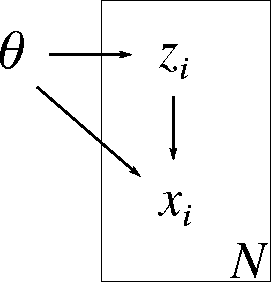
\includegraphics[height=22mm]{./figs/05-DZtheta.pdf}
\end{figure}

\subsection{Expectation Maximization}
\no Goal
\begin{itemize}
	\item Given the likelihood $P(D\;|\;Z, \theta)$, and prior on hidden variables $P(Z\;|\;\theta)$,
	\item The joint is $P(D, Z\;|\;\theta) = P(D\;|\;Z, \theta)\, P(Z\;|\;\theta)$
	\item The marginal is $P(D\;|\;\theta) = \sum_Z P(D, Z\;|\;\theta)$
	\item We wish to find $\theta$ that maximizes the marginal, i.e.
	\be
		\theta^\text{MLE} = \amax_{\theta} \Big[\log P(D \;|\; \theta)\Big] = \amax_{\theta} \left[\log \Big(\sum_Z P(D, Z\;|\;\theta)\Big)\right]
	\ee
	\item Direct numerical optimization is usually feasible, but the EM method is often faster.
\end{itemize}


\no Expectation Maximization (EM) algorithm:
\begin{enumerate}
	\item Start with realistic $\theta = \theta^\text{old}$
	\item E-step: Calculate $P(Z\;|\;D,\theta^\text{old}) = \frac{P(D, Z\;|\;\theta^\text{old})}{\sum_{Z'} P(D,Z'\;|\;\theta^\text{old})}$
	\item M-step: Find the optimal $\theta = \theta^\text{new}$ that maximizes $\sum_Z P(Z\;|\;D,\theta^\text{old})\log P(D,Z\;|\;\theta)$
	\item Set $\theta^\text{old} \leftarrow \theta^\text{new}$, check convergence, and return to E-step if needed.
\end{enumerate}

\begin{itemize}
	\item The one-liner iteration formula is based on the joint $P(D,Z\;|\;\theta)$:
	\be
		\theta^\text{new} = \amax_\theta\left[\sum_Z \frac{P(D, Z\;|\; \theta^\text{old})}{\sum_{Z'} P(D, Z'\;|\; \theta^\text{old})} \log P(D, Z\;|\; \theta)\right]
	\ee
\end{itemize}


\newpage
\subsection{Mixture models}
\begin{itemize}
	\item Data: $D=\{x_i\}_{i=1}^N$
	\item Parameters: $\theta, w$ 
		\begin{itemize}
			\item Components: $c \in \{1, 2, \ldots C\}$
			\item Parameters for each component $\theta = \{\theta_c\}_{c=1}^C$
			\item Mixing proportions: $w = \{w_c \in [0,1]\}_{c=1}^C$, such that $\sum_c w_c = 1$.
		\end{itemize}
	\item Hidden variables: labels $L = \{l_i\}_{i=1}^N$, where $l_i\in \{1, 2, \ldots C\}$
	\item Model: mixture of distinct distributions
		\begin{itemize}
			\item Generative distribution for each component: $P(x_i\;|\;l_i = c, \theta) = P(x_i\;|\;\theta_c)$
			\item Probability of an observation coming from a component: $P(l_i = c) = w_c$
		\end{itemize}
	
	\begin{figure}[h]
	\centering
		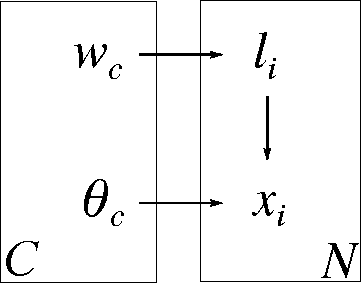
\includegraphics[height=22mm]{./figs/05-mixture.pdf}
	\end{figure}
	\item Joint
	\be
		P(D, L\;|\; \theta, w) = P(D\;|\;L, \theta) \;P(L\;|\;w) = \prod_{i=1}^N P(x_i\;|\;\theta_{l_i})\; w_{l_i}
	\ee
	\item Marginal
	\be
		P(D\;|\; \theta, w) = \sum_L P(D, L\;|\; \theta, w) = \prod_{i=1}^N\left[\sum_{c=1}^C w_c\, P(x_i\;|\;\theta_c) \right]
	\ee
\end{itemize}

\no EM algorithm
\begin{enumerate}
	\item Start with initial values: $\theta^\text{old}, w^\text{old}$
	\item In E-step, calculate
	\be	
		P(l_i = c\;|\;x_i,\theta^\text{old}) = \frac{w^\text{old}_c P(x_i\;|\;\theta^\text{old}_c)}{\sum_{c'} w^\text{old}_{c'} P(x_i\;|\;\theta^\text{old}_{c'})} =: r_{i,c}
	\ee
	\item In M-step, calculate
	\ba
		w_c^\text{new} &=& \frac{1}{N} \sum_{i=1}^N r_{i,c} 
		\\
		\theta_c^\text{new} &=& \amax_{\theta_c} \left[\sum_{i=1}^N r_{i,c} \log P(x_i\;|\;\theta_c)\right] 
		\\
		&=& \text{MLE of $\theta$ with data weights }\{r_{i,c}\}_{i=1}^N
	\ea
\end{enumerate}

\newpage
\subsection{Gaussian Mixture Model}
\no (aka. GMM or ``soft K-means clustering'')
\begin{itemize}
	\item Data: $\{x_i\}_{i=1}^N$, where $x_i \in \mathds{R}^d$ (point in $d$ dimension)
	\item Parameters:
	\begin{itemize}
		\item Clusters: $k \in \{1, 2, \ldots K\}$
		\item Mixture proportions: $\{w_k \in [0,1]\}_{k=1}^K$, where $\sum_k w_k = 1$
		\item Cluster means: $\mu = \{\mu_k \in \mathds{R}^d\}_{k=1}^K$
		\item Cluster covariances: $\Sigma = \{\Sigma_k \in \mathds{R}^{d\times d}, \text{positive definite}\}_{k=1}^K$.
	\end{itemize}
	\item Hidden variables: cluster labels, $L = \{l_i\}_{i=1}^N$, where $l_i \in \{1, 2,\ldots K\}$
	\item Model
	\ba
		P(l_i = k) &=& w_k
		\\
		P(x_i\;|\;l_i=k, \mu, \Sigma) &=& \text{Normal}(x_i\;|\;\mu_k, \Sigma_k) = \frac{1}{\sqrt{\det (2\pi \Sigma_k)}} \exp\left(-\frac{1}{2}(x_i - \mu_k)^\top (\Sigma_k)^{-1}(x_i - \mu_k)\right)
	\ea
	\item Marginal:
	\be
		P(D\;|\;\mu, \Sigma, w) = \prod_{i=1}^N\left[\sum_{k=1}^K w_k\, \text{Normal}(x_i\;|\;\mu_k, \Sigma_k)\right]
	\ee
	\item EM algorithm
	\begin{enumerate}
		\item Choose realistic $w^\text{old}, \mu^\text{old}, \Sigma^\text{old}$ initial values.
		\item In E-step, calculate
		\be
			r_{i,k} = \frac{w^\text{old}_k \,\text{Normal}(x_i\;|\;\mu^\text{old}_k,\Sigma^\text{old}_k)}{\sum_{k'} w^\text{old}_{k'} \,\text{Normal}(x_i\;|\;\mu^\text{old}_{k'},\Sigma^\text{old}_{k'})}
		\ee
		\item In M-step, calculate
		\ba
			w_k^\text{new} &=& \frac{1}{N} \sum_{i=1}^N r_{i,k} 
			\\
			\mu_k^\text{new} &=& \frac{1}{w_k^\text{new} N } \sum_{i=1}^N r_{i,k} \,x_i \\
			\Sigma_k^\text{new} &=& \frac{1}{w_k^\text{new} N } \sum_{i=1}^N r_{i,k} (x_i - \mu_k^\text{new}) (x_i - \mu_k^\text{new})^\top
		\ea
	\end{enumerate}
\end{itemize}

\newpage
\no The following python class implements the EM algorithm for fitting GMM.
\begin{lstlisting}[language=python]
class GmmEm:
    def __init__(self, x):
        self.x = np.array(x)
        self.N, self.d = self.x.shape
        self.K = None
        self.weights = None
        self.means = None
        self.covs = None
    
    def initialize(self, K):
        self.K = K
        m0 = np.mean(x, axis=0)
        cov0 = np.cov(x.T)

        self.weights = [1.0/K] * K
        self.means = multivariate_normal.rvs(mean=m0, cov=cov0, size=K)
        cov_values, _ = np.linalg.eig(cov0)
        self.covs = np.array([np.eye(self.d) * 0.1 *cov_values.max()
                             for _ in range(K)])
        
    def e_step(self):
        r = []
        for k in range(K):
            r.append(self.weights[k] * 
                     multivariate_normal.pdf(self.x, 
                                             mean=self.means[k],
                                             cov=self.covs[k]))
        r = np.array(r).T
        r_sum = np.einsum('ik->i', r)
        r = np.einsum('ik,i->ik', r, 1.0/r_sum)
        return r
    
    def m_step(self, r):
        weights_new = 1.0/N * np.einsum('ik->k', r)
        means_new = 1.0/N * \
                    np.einsum('k, ik,id->kd', 
                              1.0/weights_new, 
                              r, 
                              self.x)
        deviations = np.array([self.x - means_new[k] for k in range(self.K)])
        covs_new = 1.0/N * \
                    np.einsum('k,ik,kid,kiD->kdD', 
                              1.0/weights_new, 
                              r, 
                              deviations, 
                              deviations)
        
        self.weights = weights_new
        self.means = means_new
        self.covs = covs_new
\end{lstlisting}

\newpage
\no Example: GMM in 2D with $K=2$
\begin{figure}[h]
\centering
	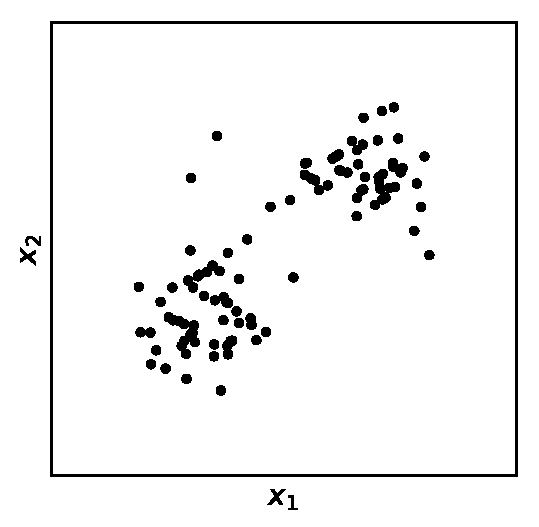
\includegraphics[width=0.30\textwidth]{./figs/05-gmm-data.pdf}
\end{figure}

\no Iterating the E- and M-steps a couple of times, we arrive to the final set of $r$ values.
\begin{lstlisting}[language=python]
gmm = GmmEm(x)

K = 2
gmm.initialize(K)
for it in range(12):
    r = gmm.e_step()
    gmm.m_step(r)
\end{lstlisting}

\begin{figure}[h!]
\centering
	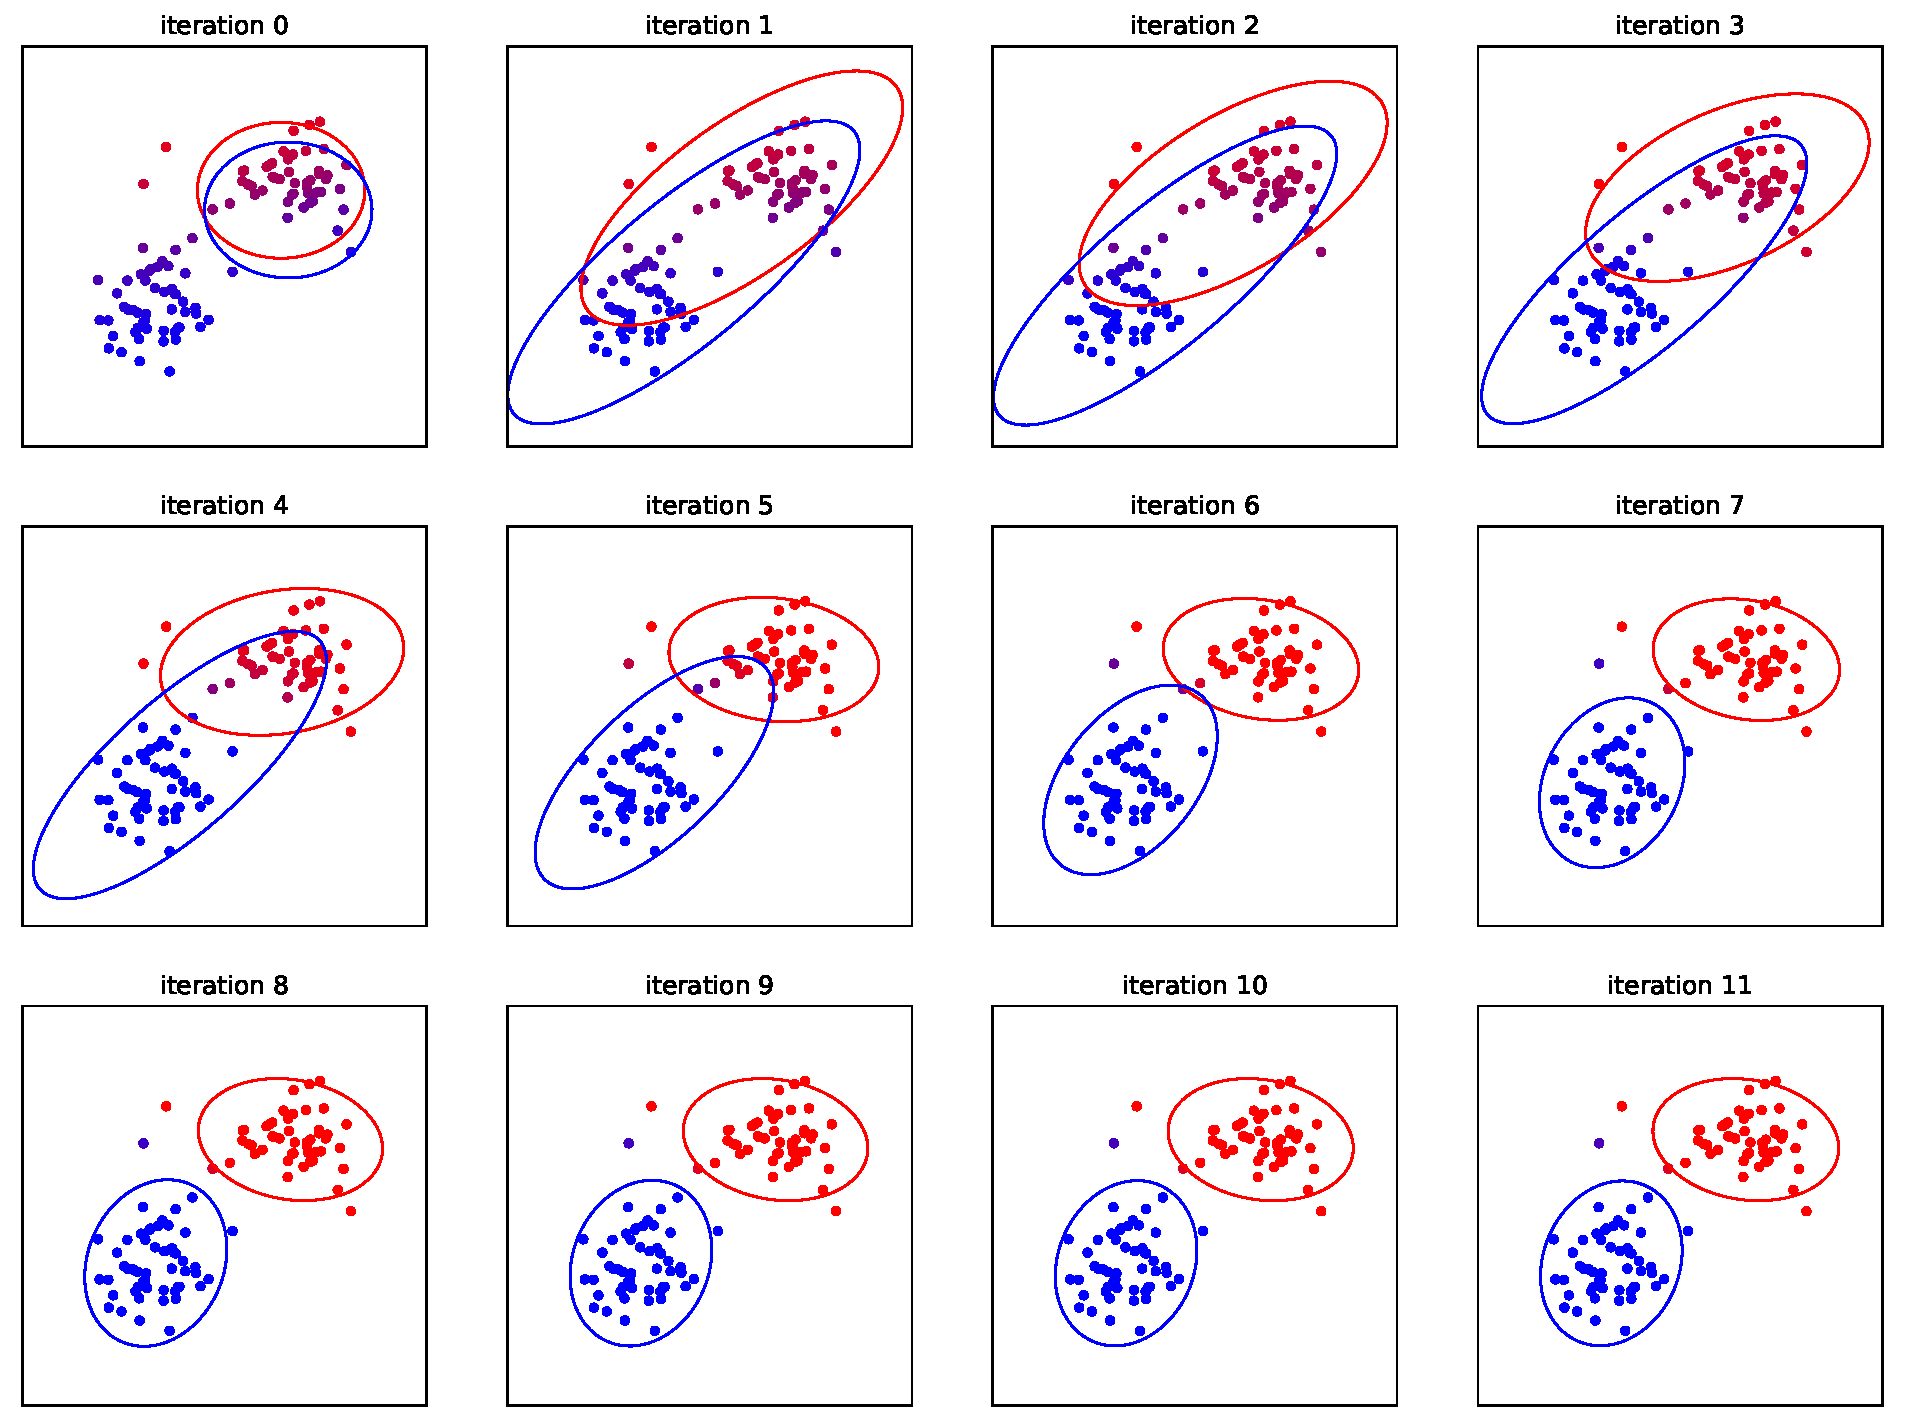
\includegraphics[width=0.93\textwidth]{./figs/05-gmm-iterations.pdf}
\end{figure}





